\documentclass[a4paper,12pt]{article}
\usepackage[utf8]{inputenc}
\usepackage[T1]{fontenc}
\usepackage[spanish]{babel}
\usepackage{csquotes}
\usepackage{anysize}
\usepackage{graphicx}
\marginsize{25mm}{25mm}{25mm}{25mm}

\title{Psychological mechanisms and the Marginal Value Theorem: effect of variability in travel time on patch exploitation}
\author{Alejandro Kacelnik \and Ian A. Todd}
\date{1992}

\begin{document}
{\scshape\bfseries \maketitle}

Para maximizar la tasa de ganancia a largo plazo los organismos deben permanecer en un parche mientras su tasa de recompensa sea mayor que la tasa global del ambiente completo (de acuerdo con el Teorema de Valor Marginal). Esta función depende de variables como el tipo de parche presente y el tiempo de viaje. En este experimento se mantendrá constante la calidad del parche pero se variará el tiempo de viaje.

Para hacer predicciones cuantitativas con base en el Teorema de Valor Marginal se deben hacer especificaciones sobre la ventana temporal sobre la cual los estimados de la tasa ``instantánea'' de ingesta y la tasa del entorno se forman. El MVT busca maximizar la tasa de ingesta en períodos largos y no en ciclos de un solo parche. Dado que el tiempo total depende de la media de tiempos de viaje pero no de su distribución, el MVT predice que las variaciones en la distribución de tiempos de viaje no tendrán ningún efecto en la política de maximización. Pero hay razones para dudar de esa predicción.

En varias tareas la memoria de las variables temporales está fuertemente relacionada con la distribución de intervalos experimentados. Cuando un animal experimenta una mezcla de intervalos construye una función de probabilidad en su memoria a largo plazo que preserva la media pero modifica la varianza y sesgo de la mezcla experimentada. Esta mezcla esa más positivamente sesgada que la mezcla experimentada. 

Modelos de decisión asumen que cuando un animal usa la memoria temporal, toma muestras de esta función en lugar de utilizar la media, por lo que la distorsión en la memoria con respecto a lo realmente experimentado afecta a la toma de decisiones. Esta discrepancia entre entre las formas de las distribuciones depende de la varianza de la mezcla experimentada, por lo que esa varianza sí afectará a las decisiones futuras. Integrar este supuesto en el MVT resulta en el modelo MVT$_{SET}$ (porque integra la teoría de expectancia escalar, SEC). Aunque este modelo es de estado estable y no menciona cómo será la dinámica de la construcción de la función de memoria.

Otra línea argumentativa indica que las demoras más recientemente experimentadas tienen un efecto desproporcionadamente grande en la toma de decisiones sobre explotación de parches. 

Con base en esto se realizan los siguientes presupuestos:

\begin{enumerate}
	\item Todos los parches son idénticos y se agotan
	\item El animal ajusta su conducta solo al esfuerzo de viaje pagado por llegar al parche actual
	\item La explotación es predicha por el MVT para un ambiente con iguales tiempos de viaje pero en el cual el animal solo usa el tiempo más reciente. La función que describe la explotación es $n = f(t)$ donde $t$ es el último tiempo de viaje y $n$ es el número de presas capturadas en cada parche. $f(t)$ es una función creciente que desacelera.
\end{enumerate}

Este modelo que solo toma en cuenta memoria para un ciclo será nombrado MVT$_{1}$. En este caso el animal maximizaría la tasa de ingesta por ciclo en lugar de a largo plazo. {\itshape Es claro que esta conducta no maximiza la tasa de ingesta a largo plazo}.

Se considera el caso en que se aplica MVT$_{1}$ a ambientes donde que se varía la dispersión de la distribución de tiempos de viaje pero se preserva la media. En el ambiente $E_{1}$ solo hay un tiempo de viaje, $\tau$. En el ambiente $E_{2}$ el forrajeador encuentra al azar dos tiempos de viaje ($\tau + \delta$ y $\tau - \delta$). La media es igual en ambos ambientes.

La media de presas por visita (PPV) en $E_{1}$ será $n_{1} = f(\tau)$, mientras que en $E_{2}$ será $n_{2} = \frac{[f(\tau + \delta) + f(\tau - \delta)]}{2}$. Dada la desigualdad de Jensen, $n_{2} < n_{1}$.

En ambientes con distribuciones uniformes simétricas de $m$ tiempos de viaje ($m > 2$) con media $\tau$ y rango $[\tau - \delta, \tau + \delta]$ la predicción es que $n_{2} < n_{m} < n_{1}$.

Ambas visiones predicen desviaciones del MVT según incrementa la varianza de tiempo de viaje, pero difieren entre sí en otros aspectos. Bajo el modelo $MVT_{1}$, un mismo tiempo de viaje en distintas distribuciones debería resultar en iguales cantidades de presas capturadas debido a que se asume que los tiempos de viaje no tienen efectos duraderos en los animales. Bajo el $MVT_{SET}$ los cambios en las presas promedio capturadas por parche se deben a distintas representaciones cognitivas del ambiente bajo las dos distribuciones de tiempos. Esto predice que habrá diferencias en un mismo tiempo de viaje proveniente de dos distribuciones distintas.

El MVT no predice varianza en PPV. Bajo $MVT_{1}$ se espera varianza proporcional a la varianza en tiempo de viaje, y bajo $MVT_{SET}$ la varianza en PPV se debe a la varianza en la memoria, y debería estar presente en todas las condiciones. Se presenta una prueba experimental de los modelos alternativos.

{\scshape\bfseries Methods}

Se utilizaron ocho palomas. Las cajas operantes tenían un panel con dos teclas de respuesta, una luz ambiental, y un comedero.

Los animales pasaron por pre-entrenamiento para picar las teclas. El color rojo anunciaría la presencia de comida, y el blanco la posibilidad de ``viajar'' entre parches (un tiempo de espera). Las palomas fueron entrenadas para picar primero a la tecla roja para recibir comida, y luego a la tecla blanca para dar acceso a la tecla roja.

En el experimento las sesiones duraban 40 ensayos o dos horas. Un ensayos tenía dos elementos: viaje y parche. Al inicio de la sesión se encendía la luz general y la tecla izquierda en blanco. Picarla cambiaba el color a verde, lo que iniciaba el componente de viaje. La luz verde permanecía encendida por su tiempo programado según la condición, y en él no había consecuencias programadas. Al final del componente de viaje se apagaba la luz verde y se encendían la luz general y la tecla en rojo parpadeante, indicando que el parche estaba disponible pero no activo. Una respuesta en la tecla roja la hacía encenderse de forma constante y encendía la tecla de viaje en blanco. El rojo contante indicaba que el parche estaba activo; el blanco, que la opción de iniciar un tiempo de viaje estaba disponible. Así, los animales tenían la opción de obtener comida o iniciar el siguiente componente de viaje.

El componente de parche era un programa de intervalo progresivo. Sus tiempos eran de 0.93, 1.8, 3.46, 6.71, 12.93, 24.97, 48.21, 92.08, y 179.71 segundos. Un máximo de nueve presas se podía obtener por parche. Si un animal llegaba a la décima entrega teórica de comida, se apagaba la luz roja para dejar solo la opción de iniciar un nuevo viaje. La cantidad óptima de presas por parche predicha por el MVT variaba en función del tiempo medio de viaje (figura 1).

\begin{figure}[ht]
        \begin{center}
                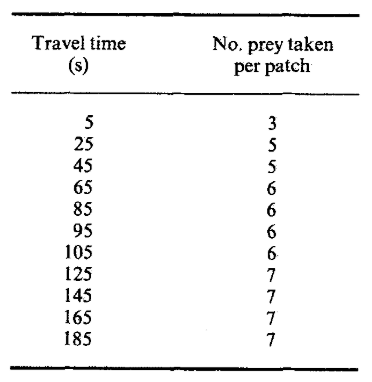
\includegraphics[scale=0.7]{Kacelnik1992(1).png}
                \caption{Cantidad óptima de presas por parche en función del tiempo promedio de viaje.}
        \end{center}
\end{figure}

Hubo tres tratamientos que diferían en el tiempo de viaje. Todos tenían una media de 95 segundos. Según el MVT, la cantidad óptima de presas en todos los casos sería de 6.

En la condición 1 (10t) hubo 10 distintos tiempos de viaje con distribución uniforme con coeficiente de variación de 60.5\%. Cada tiempo ocurrió 4 veces por sesión de forma aleatoria. En la condición 2 (2t) hubo solo dos tiempo de viaje (5 y 185 s) con coeficiente de variación de 95\%. En la condición 3 hubo  (1t) hubo solo un tiempo de viaje de 95s. El coeficiente de variación fue de cero. En las primeras 27 sesiones un grupo experimentó 2t y otro 10t, luego se revirtieron por 14 sesiones, y luego ambos pasaron por 1t.

{\scshape\bfseries Results}

{\bfseries Molar analysis.} Se calculó la PPV media en las últimas 10 sesiones de cada tratamiento individualmente para determinar el efecto de la distribución temporal. PPV fue mayor en 1t y menor en 2t, y las diferencias fueron significativas, por lo que la distribución tuvo un efecto sobre el número de presas capturadas, como predicen los modelos alternativos, aunque en este punto no son diferenciables entre sí. 

{\bfseries Molecular analysis.} Se comparó la cantidad de presas tomadas después de tiempos de viaje de 5 y 185 segundos en 2t y 10t. En ambos casos se tomaron más presas después de un tiempo largo y el incremento fue de similar magnitud. Pruebas {\scshape Anova} mostraron un efecto significativo del tiempo de viaje en el número de presas tomadas. Para descartar la posibilidad de que el efecto de debiese al tiempo previo de viaje se hizo un análisis del último tiempo de viaje (t), el penúltimo (t-1), y el antepenúltimo (t-2). Los resultados apoyaron los supuestos del modelo $MVT_{1}$. El modelo $MVT_{SET}$ no aborda la cuestión del efecto de recencia de los tiempos de viaje.

{\bfseries Variance in the data.} Bajo MVT no habría diferencias entre los tratamientos dado que su media de tiempo de viaje es la misma. $MVT_{SET}$ predice que la varianza en PPV correlacionará con la varianza en la distribución de memoria de la mezcla de tiempos de viaje. Esta distribución subjetiva debería tener varianza en los tres tratamiento a pesar de tener distintas formas. El modelo $MVT_{1}$, en el cual el número d presas recolectadas depende solo del último tiempo de viaje, predice una correlación directa entre la varianza en tiempos de viaje y varianza en PPV.

Un {\scshape Anova} mostró que la varianza en PPV era distinta entre tratamientos.

Para el modelo $MVT_{1}$ el coeficiente de variación de PPV predicho incrementa con el incremento en la variación de los tiempos de viaje experimentados. Sin embargo, aunque hubo diferencias entre tratamientos en el coeficiente de variación, no hubo una tendencia clara, sino solo una indicación leve de una respuesta a la variación incremental en tiempos de viaje.

{\scshape\bfseries Discussion}

Cuando los modelos de optimalidad de primera generación fallan pruebas empíricas, es necesario probar sus supuestos para desarrollar versiones más detalladas. Este experimento en especial se realizó porque, con base en conocimiento externo sobre mecanismos conductuales, se esperaba que las predicciones del MVT estuviesen mal. Esta información vino de mecanismos psicológicos de procesamiento de información ($MVT_{SET}$) y de estudios de tiempo de viaje en MVT. Ambas líneas llevaron a esperar un menor numero de presas recolectadas por parche comparadas con las predicciones de MVT.

Estos resultados no permiten generar un modelo más específico debido a que se desprecian los costos de viaje (los animales no gastan energía extra por esperar), pero sirven para examinar los supuestos de las dos líneas de razonamiento.

El análisis molecular confirma en general el supuesto de $MVT_{1}$ (solo el último tiempo de viaje debe afectar la decisión). Pero el número de presas recolectadas fue sensible a la mezcla de tiempos de viaje, de modo que memoria más allá del último tiempo de viaje debió afectar. Además, hubo varianza considerable en las presas capturadas aun cuando no había varianza programada en tiempo de viaje, por lo que la varianza conductual no puede explicarse enteramente por la varianza en el ambiente.

El modelo $MVT_{SET}$ en su forma actual no hace predicciones sobre la correlación entre las varianzas en la conducta y la experiencia. Pero predice que la mezcla de tiempos de viaje (y no solo el último) debería tener un efecto entre tratamientos, y predice varianza en todos ellos. Así, no se puede rechazar el modelo de memoria escalar.

El estudio ilustra que los modelos de optimalidad sirven como un marco de referencia para la integración de hipótesis causales y funcionales, y resaltan las características de la conducta que necesitan de una explicación.

La teoría de forrajeo no puede desarrollarse en ausencia de datos empíricos.

Parece ser que las palomas y los {\itshape starlings} se desvían de las predicciones basadas en la maximización a largo plazo debido a sus limitaciones de memoria.


\end{document}
